\subsection{Архитектура РСУБД}

Есть программа, есть данные, и программа обращается к данным.

\paragraph{Протокол} Для взаимодействия нужен протокол, его реализуют драйвера, которые находятся
и на стороне программы, и на стороне СУБД, которая уже будет обращаться в хранилище. Могут быть
различные протоколы, традиционно у каждого субд есть свой протокол, по которому можно с ней
общаться

\begin{remark}
	СУБД и хранилище находятся на одном компьютере, благодаря этому нет передачи данных по сети во
	время исполнения запроса (если хранилище представляет из себя несколько компьютеров то
	взаимодействие по сети всё же есть).
\end{remark}

\paragraph{Запрос}
\begin{enumerate}
	\item Стандартный SQL запрос требуется разобрать, для этого есть модуль \textit{Разборщик запроса}, который
	      представляет из себя парсер.
	\item \textit{Исполнитель запроса} исполняет запрос, но так как исполнять ровно тот запрос
	      который написан не эффективно существует \textit{Оптимизатор}.
	\item \textit{Посторитель плана исполнения} или \textit{Оптимизатор} берёт разобранный
	      запрос и решает как он будет исполняться: какие, откуда и в каком порядке будут загружаться данные,
	      какие индексы будут использованы.
	\item Управление памятью - это важно для исполнителя, потому что от того поместятся все данные в память
	      или нет зависит эффективная реализация запроса.
	\item Статистика. Например нам нужно прочитать данные о всех студентах конкретного пола, либо мальчиков,
	      либо девочек, тогда имея статистику и том что их кол-во отличается на порядок оптимизатор может
	      понять что всех мальчиков будет быстрее прочитать просто читая все данные подряд, а девочек,
	      возможно при наличии способа быстро идентифицировать именно девушек, читая данные только о них.
\end{enumerate}

\begin{figure}[H]
	\centering
	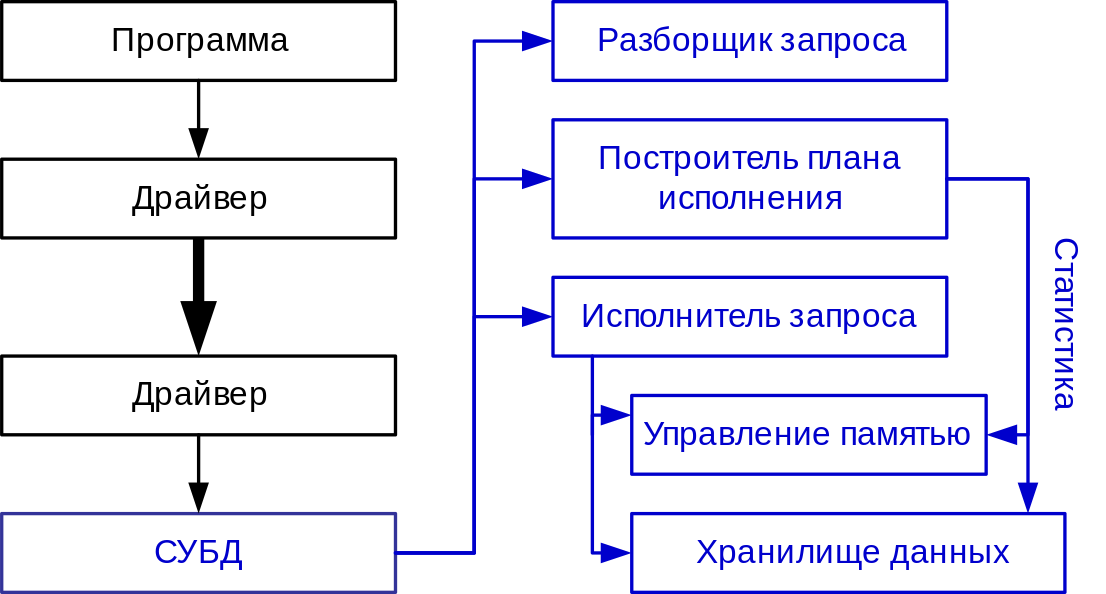
\includegraphics[width=0.8\textwidth]{../assets/kgeorgiy/intro/intro_arch_complete.svg.png}
	\caption{Полноценная схема}
	\label{rsubd-scheme}
\end{figure}
